%%% The main file. It contains definitions of basic parameters and includes all other parts.


%% Settings for two-sided (duplex) printing
\documentclass[10pt,a4paper]{report}
\let\openright=\cleardoublepage

%% Character encoding: usually latin2, cp1250 or utf8:
\usepackage[utf8]{inputenc}

%% It's 2019
\usepackage[default]{droidserif}
\usepackage[T1]{fontenc}

%% Further useful packages (included in most LaTeX distributions)
\usepackage{amsmath}        % extensions for typesetting of math
\usepackage{amsfonts}       % math fonts
\usepackage{graphicx}       % embedding of pictures
\usepackage{tikz}
%\usetikzlibrary{shapes,fit,positioning,snakes,mindmap,trees,decorations.text,arrows.meta}
%\makenomenclature
\usepackage{algorithm,algpseudocode}
\usepackage{booktabs}
\usepackage{mwe}
\usepackage{pgfgantt}
\usepackage{pdflscape}
\usepackage{geometry}
\usepackage{enumitem}
\usepackage{float}
\usepackage{framed}
\usepackage{titlesec}
\usepackage{listings}
\usepackage{xcolor}
\usepackage{longtable}

\usepackage{multirow}

\lstset{basicstyle=\ttfamily,
	showstringspaces=false,
	commentstyle=\color{red},
	keywordstyle=\color{blue}
}

\usepackage{pdfpages}

\usepackage[textsize=tiny,backgroundcolor=yellow!50, linecolor=black!25]{todonotes}

% links shall be clickable
\usepackage[unicode]{hyperref}   % Must follow all other packages
\usepackage{cleveref} % Must follow all other packages including hyperref

% Definitions of macros (see description inside)

\newcommand{\cool}{\color{green!50!white!80!black}}
\newcommand{\textcool}[1]{{\cool #1}}

\newcommand{\XX}[1]{\textcolor{red}{#1}}
\newcommand{\TT}[1]{\texttt{#1}}
\newcommand{\SC}[1]{{\fontfamily{phv}\selectfont\textsc{#1}}}

% Draw black "slugs" whenever a line overflows, so that we can spot it easily.


% avoid some slugs naturally
\clubpenalty=1000
\widowpenalty=1000
%\hyphenpenalty=100  % turn this on to prevent hyphenation
\emergencystretch=2cm


%%% The field of all real and natural numbers
\newcommand{\R}{\mathbb{R}}
\newcommand{\N}{\mathbb{N}}
\newcommand{\F}{\mathbb{F}}
\newcommand{\Z}{\mathbb{Z}}

\newcommand{\bms}{\begin{enumerate}[label=\bf (M\arabic*)]}
\newcommand{\bwp}{\begin{enumerate}[label=\bf \normalsize  (WP\arabic*), resume=del]}
\newcommand{\eenum}{\end{enumerate}}
\newcommand{\itemm}{\large \item }
\newcommand{\itemwp}{ \normalsize \item }
\newcommand{\deadline}[2]{\small (deadline: \textit{month #1}, duration: \textit{#2 moths})}
\newcommand{\people}[1]{\textit{\small (#1)}}


% move the headings out of gutenberg era
\setcounter{secnumdepth}{4}
\titleformat{\chapter}{\cool\fontsize{24pt}{24pt}\bfseries}{\color{black!25}\thechapter.}{1em}{}
\titleformat{\section}{\cool\fontsize{16pt}{18pt}\bfseries}{\scriptsize\color{black!25}\thesection}{1em}{}
\titleformat{\subsection}{\cool\fontsize{14pt}{16pt}\bfseries}{\scriptsize\color{black!25}\thesubsection}{1em}{}
\titleformat{\subsubsection}{\cool\fontsize{12pt}{14pt}\bfseries}{\scriptsize\color{black!25}\thesubsubsection}{1em}{}

% code floats
\colorlet{shadecolor}{cyan!10}
\makeatletter
\newcommand\floatc@code[2]{{\@fs@cfont #1} #2\par}
\newcommand\fs@code{\def\@fs@cfont{\bfseries}\let\@fs@capt\floatc@code
\def\@fs@pre{}%
\def\@fs@mid{\vspace{-.5ex}\begin{shaded}}%
\def\@fs@post{\vspace{-1em}\end{shaded}}%
\let\@fs@iftopcapt\iftrue}
\makeatother

\floatstyle{code}
\newfloat{listing}{tbp}{lst}
\floatname{listing}{Listing}


\title{\textcool{\bf High Level Assembler Plugin} \\ Project specification}
\author{Michal Bali, Marcel Hruška, Peter Polák,\\ Adam Šmelko, Lucia Tódová}
\date{Supervisor: Miroslav Kratochvíl}

% Title page and various mandatory informational pages
\begin{document}
\maketitle

%%% A page with automatically generated table of contents of the bachelor thesis

\tableofcontents

%%% Each chapter is kept in a separate file
\chapter{Introduction}

The IBM High Level Assembler Language (HLASM) is still actively used commercially, even though it is a relatively old language. Its roots go back to the 1970s, when IBM made their first mainframes. Since then, the IBM assembler has been revised several times --- the last version (which is the concern of this project) was released in 1992. Although it is hard to believe, a lot of the software that has been written in the language over the years is still actively used and maintained, mainly because of the conservative mainframe users and IBM's vendor lock-in.

Today, HLASM developers are forced to code in archaic terminals directly on the mainframe. Therefore, they spend a lot of time navigating around the code and the environment. For example, solely due to the fact that the user needs to navigate through plenty of terminal screens it takes around a minute just to get to a screen where it is possible to make a change in a file and recompile. For developers, it would be extremely useful to have an IDE plugin that would minimize contact with the mainframe terminal, could analyze the HLASM program, check its validity and make the code clearer by syntax highlighting. 

We introduce such plugin for Visual Studio Code, which is nowadays one of the most popular code editors. It improves HLASM programming experience, so that it can be compared to coding in modern programming languages, by providing instant code validity checks, advanced highlighting, code analysis, and all the functionality that a programmer currently takes for granted when writing code.

Some of the most noteworthy properties and features of the plugin are:
\begin{itemize}
	\item It is capable of interpreting and tracing a large subset of HLASM code-generating instructions
	\item It contains a list of all built-in instructions that is used to validate the generated code
	\item So called \emph{macro tracer} gives a possibility to trace the compilation of HLASM source code step-by-step in a way similar to common debugging.
	\item It implements DAP and LSP protocols, providing interface to be easily integrated into numerous modern code editors
	\item It has been run and tested on over 15 millions lines of real production HLASM code
\end{itemize}
The plugin is available on the Visual Studio Code Marketplace\footnote{\url{https://marketplace.visualstudio.com/items?itemName=broadcomMFD.hlasm-language-support}}

This document serves as an in-depth documentation for anyone who would like to understand the implementation of the project and the reasons behind it. It is advised that the potential contributors to the project read this documentation first.

User documentation is available on the Visual Studio Code marketplace \footnote{\url{https://marketplace.visualstudio.com/items?itemName=broadcomMFD.hlasm-language-support}} or in a markdown file \TT{clients/vscode-hlasmplugin/README.md}. The HLASM plugin project also contains an example workspace that can be used to test out the plugin.


\section{Organisation of this document}
First of all, in~\cref{hlasm}, we briefly explain the basics of HLASM needed to comprehend the workflow of this language. In~\cref{arch}, we provide an overview of the project's architecture, naming the most important components and indicating their relations. Then, we describe these components in separate chapters in further detail. In~\cref{chap:lang_server}, we state the responsibilities of the language server as the communication provider between the extension client and the parsing library. The workspace manager is the entry point to the parsing library used by the language server and it is fully described in~\cref{ws_manager}. The purpose of its sub-components is to handle file management, dependency resolution and parsing. The core of the processing of a HLASM file is implemented inside the analyzer, whose mechanics and implementation details are discussed in~\cref{chap:analyzer}. The project also provides macro tracing through the standard debugging procedure and it is fully explained in~\cref{macro_tracer}.The last mentioned component, detailed in~\cref{extension} is the VSCode extension, which communicates with the language server and provides IDE features to the user. At the end of this document, in~\cref{build}, we provide the instructions on how to build the project.

\chapter{HLASM overview}
\label{hlasm}
Ordinary assembly languages consist solely of ordinary machine instructions. High-level assemblers generally extend them with features commonly found in high-level programming languages, such as control statements similar to \emph{if, while, for} as well as custom callable macros.

IBM High Level Assembler (HLASM) satisfies this definition and adds other features, which will be described in this section.

\section{Syntax}

HLASM syntax is similar to a common assembler, but due to historical reasons it has limitations, like line length limited to 80 characters (as that was the length of a punched card line).

\subsection{Statement}

HLASM program consists of a sequence of \emph{statements}, which are used to produce both compile-time code and run-time code (see \cref{Assembling}). A statement consists of four fields separated by spaces that can be split into more lines using continuations (see \cref{Continuation}). Following are the existing fields:
\begin{itemize}
	\item \textbf{Name field} --- Serves as a place for named constants that are to be used in the code. This field is optional, but, when present, it must start at the begin column of a line.
	
	\item \textbf{Instruction field} --- The only mandatory field, represents the instruction that is executed. It must not begin in the first column, as it would be interpreted as a name field.
	
	\item \textbf{Operands field} --- Field for instruction operands, located immediately after instruction field. Individual operands must be separated by a comma, and, depending on the specific instruction, can be either blank, in a form of an apostrophe separated string, or represented by a sequence of characters.
	
	\item \textbf{Remark field} --- Optional, serves as inline commentary. Located either after the operands field, or, in case the operands are omitted, after the instruction field. 
\end{itemize}

\begin{listing}[t]
	\begin{verbatim}
name    instruction     operands             remark
.NOMOV       AGO     (&WH).L1,.L2,.L3     SEQUENTIAL BRANCH
	\end{verbatim}
	\caption{An example statement.}
	\label{lst:small_example}
\end{listing}

\Cref{lst:small_example} shows an example of a basic statement containing all fields.

\subsection{Continuations}
\label{Continuation}

Individual statements sometimes contain more than 80 characters, which does not agree with the historical line length limitations. Therefore, a special feature called \emph{continuation} exists.

For this purpose the language specification defines four special columns:
\begin{itemize}
	\item \emph{Begin column} (default position: 1)
	
	\item \emph{End column} (default position: 71)
	
	\item \emph{Continuation column} (default position: 72)
	
	\item \emph{Continue column} (default position: 16)
\end{itemize}

The begin column defines where the statements can be started.

The end column determines the position of the end of the line. Anything written to its right does not count as content of the statement, and is rather used as a line sequence number (see \cref{fig01:line}).

The continuation column is used to indicate that the statement continues on the next line. For proper indication, an arbitrary character other than space must be written in this column. The remainder of the statement must then start on the continue column.

An example of an instruction where its last operand exceeded column 72 of the line can be seen in \cref{lst:overflow}.

\begin{listing}[t]
	\begin{verbatim}
    OP1                            REG12,REG07,REG04,REG00,REG01,REG11,Rx
                EG02
	\end{verbatim}
	\caption{Example program that uses the continuation to write a statement longer than 80 characters.}
	\label{lst:overflow}
\end{listing}

Some instructions also support the \emph{extended format} of the operands. This allows the presence of a continuation character even when the contents of a line have not reached the continuation column (see \cref{lst:extended}).

\begin{listing}[t]
	\begin{verbatim}
          AIF   ('&VAR' FIND '~').A,     REMARK1                        x
                ('&VAR'  EQ  'L').B,     REMARK2                        x
                (T'&VAR  EQ  'U').C      REMARK3 
	\end{verbatim}
	\caption{Extended instruction format.}
	\label{lst:extended}
\end{listing}

\begin{figure}
	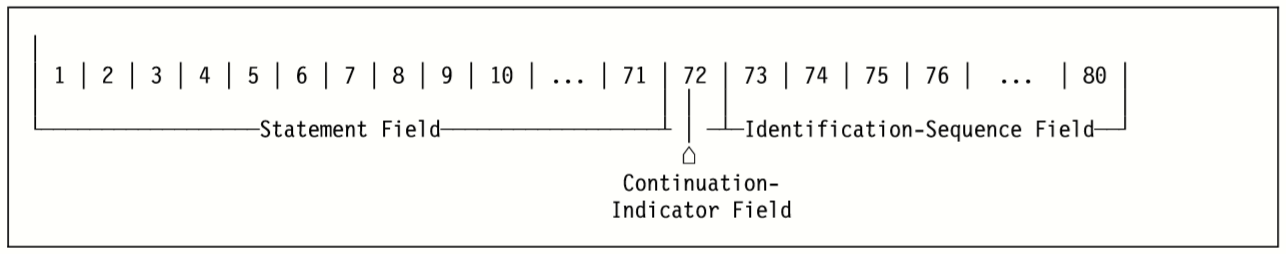
\includegraphics[width=\textwidth]{img/line}
	\caption{Description of line columns (source: \href{https://www-01.ibm.com/servers/resourcelink/svc00100.nsf/pages/zOSV2R3sc264940/$file/asmr1023.pdf}{HLASM Language Reference} ).}
	\label{fig01:line}
\end{figure}


\section{Assembling}
\label{Assembling}

Having briefly outlined the syntax, we now describe the assembly process of HLASM. 

We distinguish two types of processing:

\begin{itemize}
	\item \emph{conditional assembly (CA) processing} --- the main purpose of which is to generate statements for ordinary assembly (see \cref{CA_proc})
	\item \emph{ordinary assembly processing} --- which handles \emph{machine instructions} and \emph{assembler instructions} (see \cref{mach_instr}, \cref{asm_instrs})
\end{itemize}

\subsection{Ordinary assembly}

Ordinary assembly, along with machine and assembler instructions, is responsible for the runtime behavior of the program. It allows the generation of code from both traditional machine instructions and special-purpose assembler instructions. Moreover, it assigns values to \emph{ordinary symbols}.

\subsubsection{Ordinary symbols}
\label{ord_sym}

In HLASM, an \emph{ordinary symbol} is a named run-time constant. It is defined by inputting its name into the name field of a statement along with a special assembler instruction. Each ordinary symbol can only be defined once, and its value is constant. There are two types of ordinary symbols:
 
\begin{itemize}
	\item An \emph{absolute symbol} that simply has an integral value.
	\item A \emph{relocatable symbol} that represents an address in the resulting object code. A relocatable symbol can also be defined by writing the ordinary symbol name into the name field of a statement along with a machine instruction name. The symbol then denotes the address of the given instruction.
\end{itemize}

In addition to symbol value, ordinary symbols also contain a set of \emph{attributes}, the most common ones being \emph{type} and \emph{length}.

\subsubsection{Machine instructions}
\label{mach_instr}

\emph{Machine instructions} represent the actual processor instructions executed during run-time. Similarly to traditional assemblers, they are translated into corresponding opcodes and their operands are processed. However, HLASM also allows expressions to be passed as their operands, which may use ordinary symbols and support integer and address arithmetic.

\subsubsection{Assembler instructions}
\label{asm_instrs}

In addition to machine instructions, HLASM assembler also provides \emph{assembler instructions} (in other systems commonly termed \emph{directives}). They instruct the assembler to make specific actions rather than to assemble opcodes. For example, they generate run-time data constants, create ordinary symbols, organize the resulting object code and generally affect how the assembler operates.

Following are examples of assembler instructions:
\begin{itemize}
	\item \textbf{ICTL} --- Changes values of the previously described line columns (i.e. begin column may begin at column 2 etc.).
	
	\item \textbf{DC}, \textbf{DS} --- Reserves space in object code for data described in operands field and assembles them in place (i.e. assembles float, double, character array, address etc.). These instructions take \emph{data definition} as operands. \Cref{data_def_example} shows examples of data definition.
	
	\item \textbf{EQU} --- Defines ordinary symbols.
	
	\item \textbf{COPY} --- Copies text from a specified file\footnote{Path to the folder of the file is passed to assembler before the start of assembly} (called \emph{copy member}) and pastes it in place of the instruction. It is very similar to the C preprocessor \texttt{\#include} directive.
	
	\item \textbf{CSECT} --- Creates an executable control section, which serves as the start of relative addressing. It is followed by sequence of machine instructions.
\end{itemize}

\begin{figure}[t]
	\begin{verbatim}
CL8'ABC'
    C is type of data definition - array of characters
    L8 specifies length - 8 bytes
    'ABC' is nominal value of the data definition
    CL8'ABC' would assemble 8 bytes, first three of which would be EBCDIC
             representations of letters A, B and C

5AY(A+4,B)
    5 is duplication factor - the nominal value will be repeated 5 times
    A is type - address
    Y is type extension - it modifies the length of the address
    (A+4,B) is nominal value - comma separated expressions that will
            be assembled as addresses
    5AY(A+4,B) would assemble total of 20 bytes, first 2 bytes is value
               of expression A+4, then B and then 4 more copies of the same
	\end{verbatim}
	\caption{Examples of data definition}
	\label{data_def_example}
\end{figure}

\subsubsection{Ordinary symbols resolution}
\label{ordinary_resolution}
All the assembler instructions and ordinary symbols must be resolved before the assembler creates the final object file. However, as the HLASM language supports forward declaration of ordinary symbols, the assembly may be quite complicated. Consider an example in \cref{lst:ordinary_assembly}. When the instruction on line 1 is seen for the first time, it is impossible to determine its length, because the symbol \verb|LEN| is not defined yet \footnote{Character L with an expression in parentheses in DS operand of type C specifies how many bytes should be reserved in the program.}. The same applies to the length of the instruction on the second line. Furthermore, it is also impossible to determine the exact value of relocatable symbols \verb|ADDR| and \verb|HERE| because of the unknown length of the preceding instructions.

\begin{listing}[t]
	\begin{Verbatim}[numbers=left]
           DS    CL(LEN)
ADDR       DS    CL(SIZE)

HERE       DS    0H
LEN        EQU   HERE-ADDR
SIZE       EQU   1
	\end{Verbatim}
	\caption{A sample program that shows that symbols can be used prior to their definition.}
	\label{lst:ordinary_assembly}
\end{listing}


In the next step, \verb|LEN| is defined. However, it cannot be evaluated, because the subtraction of addresses \verb|ADDR| and \verb|HERE| is dependent on the unknown length of instruction on second line and therefore on the symbol \verb|SIZE|. The whole program is resolved only when the assembly reaches the last line, which defines the length of instruction \verb|02|. Afterwards, it is possible to resolve \verb|LEN| and finally the length of instruction \verb|01|.

The dependency graph created from these principles can be arbitrarily deep and complicated, however it must not contain cycles (a symbol must not be transitively dependent on itself).

\subsection{Object file layout}

The product of ordinary assembly is an object file. Let us briefly describe its layout.

\subsubsection{Sections}

An object file consists of so-called \emph{sections}. They are user-defined (by instructions CSECT, DSECT, \ldots) and can be of different kinds, each with various properties. Absolute positions of sections within the object file are undefined --- they are determined automatically after the compilation. This also implies that all relocatable symbols are only defined relatively to the section that contains them.

\subsubsection{Location counter}
\label{loctr}

Any time a machine instruction is encountered, its opcode is outputted to the \emph{next available address}. Each section has a structure pointing to this address --- a so-called \emph{location counter}.

The user may define more location counters and then arbitrarily switch between them to state the next address for code generation. Therefore, at all times, there is one and only one location counter active, which defines where the next machine instruction will be generated.

At the end of assembly, all code denoted by location counters is assembled in a well-defined order, and so the absolute position of all relocatable symbols within their section is known.

The value of the location counter can be arbitrarily changed by the ORG instruction. It can be moved backwards or forwards (with restriction of counter underflow) to set the next address. This means that user can generate some code, move counter backwards and overwrite it. Then the ORG instruction can be used to set location counter to the next available untouched address to continue in object creation.

\subsection{Conditional assembly}
\label{CA_proc}

Conditional assembly is another feature provided by HLASM. It is essentially a macro-language built on top of a traditional assembler.

User may use conditional assembly instructions to either define \emph{variable symbols}, which can be used in any statement to alter its meaning, or to define \emph{macros} --- reusable pieces of code with parameters. Based on these instructions, conditional assembly then alters the textual representation of the source code and selects which lines will be processed next.

\subsubsection{Variable symbols}
\label{var_sym}`
Variable symbols serve as compile-time variables. Statements that contain them are called \emph{model statements}.

During conditional assembly, variable symbols are substituted for their value to create a statement processable by ordinary assembly. For example, a user can write a variable symbol in the operation field and generate any instruction that can be a result of a substitution.

Variable symbols also have notion of their type --- they can be defined either as integer, boolean or string. CA instructions gather this information for different sorts of conditional branching.

\subsubsection{CA instructions}
\label{ca_instr}

CA instructions are not assembled into object code. They are used to select which instructions will be processed by the assembler next.

One example of their capabilities is conditional and unconditional branching. As HLASM provides a variety of built-in binary or unary operations on variable symbols, complex conditional expressions can be created. This is important in HLASM, as the user can alter the flow of instructions that will be assembled into an executable program.

Another subset of CA instructions operates on variable symbols. These can be used to define variable symbols locally or globally, assign or update their values.

\subsubsection{Macros}

A \emph{macro} is a structure consisting of a \emph{name}, \emph{input parameters} and a \emph{body}, which is a sequence of statements. When a macro is called in a HLASM program, each statement in its body is executed. Both nested and recursive calls of macros are allowed. Macro body can also contain CA instructions, or even a sequence of instructions generating another macro definition. With the help of variable symbols, HLASM has the power to create custom, task specific macros.

\vspace{5mm}

An example of a simple HLASM program with the description of its statements is shown in \cref{lst:example}.

On lines \verb|01-04|, we see a \emph{macro definition}. It is defined with name \verb|GEN_LABEL|, variable \verb|NAME| and contains one instruction in its body, which assigns the current address to the label in \verb|NAME|.

On line \verb|06|, the \emph{copy instruction} is used, which includes the contents of the \verb|REGS| file.

Line \verb|08| establishes a start of an executable section \verb|TEST|. 

On line \verb|09|, an integer value is assigned to a variable symbol \verb|VAR|. The value is the length attribute of previously non-defined constant \verb|DOUBLE|. The assembler looks for the definition of the constant to properly evaluate the conditional assembly expression. In the next line, there is a CA branching instruction \verb|AIF|. If value of \verb|VAR| equals 4, all the text between \verb|AIF| and \verb|.END| is completely skipped and assembling continues on line \verb|18|, where the branching symbol \verb|.END| is located.

Lines \verb|12-13| show examples of machine instructions that are directly assembled into object code. Lines \verb|11| and \verb|14| contain examples of a macro call.

On line \verb|15|, the constant \verb|LEN| is assigned the difference of two addresses, which results in absolute ordinary symbol. This value is next used to generate character data.

Instruction \verb|DC| on line \verb|17| creates value of type double and assigns its address to the ordinary symbol \verb|DOUBLE|. This constant also holds information about length, type and other attributes of the data.  

\verb|ANOP| is an empty assembler action which defines the \verb|.END| symbol and line \verb|19| ends the assembling of the program. 

%\let\oldv\verbatim
%\let\oldendv\endverbatim

%\def\verbatim{\par\hspace{1cm}\setbox0\vbox\bgroup\oldv}
%\def\endverbatim{\oldendv\egroup\fboxsep0pt \colorbox[gray]{0.8}{\usebox0}\par}

\begin{listing}[t]
    \begin{verbatim}
name        operation   operands
    \end{verbatim}
	\begin{Verbatim}[numbers=left]
            MACRO                   
&NAME       GEN_LABEL
&NAME       EQU         *
            MEND
        
            COPY        REGS
        
TEST        CSECT
&VAR        SETA        L'DOUBLE
            AIF         (&VAR EQ 4).END
LBL1        GEN_LABEL
            LR          3,2
            L           8
LBL2        GEN_LABEL
LEN         EQU         LBL2-LBL1
            DC          (LEN)C'HELLO'
DOUBLE      DC          H'-3.729'
.END        ANOP
            END
	\end{Verbatim} 
	\caption{An example of an artificial HLASM program.}
	\label{lst:example}
\end{listing}

\vspace{5mm}

Although CA processing may act like text preprocessing, it is still interlinked with ordinary processing. CA has mechanics that allow the assembler to gather information about statements that are printed during the processing. It can also access values created in ordinary assembly and use them in conditional branching, and is able to lookup constants that are not yet defined prior to the currently processed statement. During ordinary assembly, names of these instructions can also be aliased.

To sum up, CA processing has variables for storing values during the compilation and CA instructions for conditional branching. Hence, it is Turing-complete while still evaluated during compile-time.

\section{HLASM source structure}

The file that generates the object code is called an \emph{open-code} file. It is the entry file of the HLASM compiler. Each open-code file can have in-file dependencies, specifically:
\begin{itemize}
	\item External Macro definitions
	\item Copy members
\end{itemize}
These are not treated as open-code files because they do not directly generate object code. Rather, they serve as statement sequences that are included in specific places of open-code and provide specific meaning.



\chapter{Project scope}

This chapter reviews the specific goals of our project.
All the features below have been discussed with professional HLASM developers and have been agreed on by the company.

This project aims to produce a VS Code extension, downloadable from the Market Place.\todo{link} The extension contains all executables/libraries that are needed for the project to work correctly on the most popular platforms. No other prerequisites should be required.

Modularity of the software is another important requirement. 

The project implementation provides 2 kinds of API: a complex one that mirrors the Language Server Protocol\footnote{\url{https://microsoft.github.io/language-server-protocol/}} (LSP) specification and a simple one that accepts a text along with a dependency-resolver object and returns diagnostics. 

The language server implements the LSP standard, hence it can be easily reintegrated within other IDEs such as Eclipse Che.

\section{Supported language features}
\label{LSPFeatures}
This part provides a brief overview of the parts of HLASM that should be included in the final software.

\begin{description}
\item [Syntax Parser] The parser recognizes the syntax of HLASM and processes it into predefined structures. 

\item [High-level interpretation] The library interprets high-level parts of the assembler. Following are the conditional assembly instructions for code generation and macro expansion:
\begin{itemize}
    \item AIF
    \item AGO
    \item MACRO, MEND, MEXIT
    \item ACTR
    \item SETA, SETB, SETC
    \item ANOP
    \item LCLA, LCLB, LCLC
    \item GBLA, GBLB, GBLC
    \item AEJECT
    \item ASPACE
\end{itemize}
and assembler instructions for code layout determination:
\begin{itemize}
    \item EQU 
    \item DC 
    \item DS 
    \item DSECT, CSECT, RSECT 
    \item LOCTR
\end{itemize}

\item [Code Validation] The back-end semantically and syntactically checks all instructions (including machine instructions) for correct operand format usage. However, it does not analyze the run-time register and memory values, as there is no machine instruction interpretation.

\item [Dependency Search] Usage of external files in HLASM is a highly common phenomenon. On mainframes, HLASM programs are built according to its JCL\footnote{Job Control Language, instructs the system how to run a specific task} file, which contains a list of libraries. When the compiler encounters an undefined instruction or a \texttt{COPY} instruction, it does a top-down search through the whole list. Both ways of invoking a dependency search are demonstrated in \cref{lst:search}. As a large portion of the programs use the same libraries, defining these JCL files gets repetitive. Therefore, the build and source management system Endevor creates an abstraction above the libraries and groups them into \texttt{processor groups}. As a result, JCL offers an option to identify the libraries to be included by their processor group's ID instead of listing them all manually.

We adapt this system to our needs and define 2 configuration files. The first one mirrors the behavior of Endevor and defines the processor groups. The second one matches the source codes to these processor groups.

\item [Continuation Handling] Fixed-size lines are another aspect of HLASM that needs to be handled. They make the parsing more difficult, as the position of the continuation character may vary. 

We also add a continuation handling option to the IDE, which mostly consists of non-movable continuation characters, i.e. if the user types in front of the continuation character, it stays in place.

\item [Macro Tracer] To trace the code generation, the user can step through the code while watching the contents of variables and the call stack using \texttt{Macro tracer}. We implement \texttt{Debug Adapter Protocol} so that the process ressembles standard debugging. This tool is extremely useful as tracing the macro expansions manually gets tedious quickly.
\end{description}

\pagebreak
\begin{listing}
\begin{verbatim}
        MAC1       1,1                   
        COPY       COPY1
\end{verbatim} 
\caption{An example of both ways the HLASM program may invoke dependency search.}
\label{lst:search}
\end{listing}

\section{Supported LSP features}
This section demonstrates the possible uses of the extension on the client side. LSP provides a list of well-defined features. The project implements the following:

\begin{itemize}
	\item \texttt{Go to definition} command for all symbols, macro definitions and copy members\footnote{Copy, along with macro expansion, is a mean to include another external file, invoked by \texttt{COPY} instruction. Comparing to macro, copy does not neither need to start nor end with any specific instruction and the invoking \texttt{COPY} instruction is simply replaced by the COPY file's contents.}
	\item \texttt{Find all references} command for all symbols, macro definitions and copy members
	\item Completion for instructions, defined symbols and macros
	\item Mouse-over tooltip (hover) for symbol attributes, their locations, contents and other useful information depending on the symbol type
	\item Diagnostics for syntax and semantic errors and warnings
	\item Server-side Highlighting for all symbols which is our custom extension of LSP  
\end{itemize}

The highlighting is not a standard part of the LSP, nonetheless it is a needed addition. Due to the complexity of HLASM, a typical syntax highlighting is not sufficient. Consider following examples:

\lstdefinelanguage{HLASM}{
    keywords = [1]{REMARK},
    keywords = [2]{SAM31,LR,AGO,AIF,ICTL},
    keywords = [3]{J,SYMBOL},
     keywords = [4]{IGNORED},
     keywords = [5]{X},
    keywordstyle = [1]\color{blue},
    keywordstyle = [2]\color{red},
    keywordstyle = [3]\color{white},
    keywordstyle = [4]\color{magenta},
    keywordstyle = [5]\color{cyan}
}
\lstset{
numbers=left, 
numberstyle=\small, 
numbersep=8pt, 
frame = single, 
language=HLASM, 
framexleftmargin=15pt,
backgroundcolor = \color{lightgray}
}
\begin{itemize}
    \item The language server recognizes operand formats of different instructions. The most simple example is the \texttt{SAM31} instruction, which does not have any operands, while the \texttt{LR} instruction takes two. So the identifier right after \texttt{SAM31} is colored blue as a remark. 
    
\begin{lstlisting}
    SAM31 REMARK
    LR    1,1   REMARK
\end{lstlisting}

\item The code skipped by the conditional assembly is not colored and stays white.
\begin{lstlisting}
    AGO .HERE
    J   SYMBOL
.HERE AIF
\end{lstlisting}

\end{itemize}


\chapter{Architecture overview}
\label{arch}

\begin{figure}
	\centering
	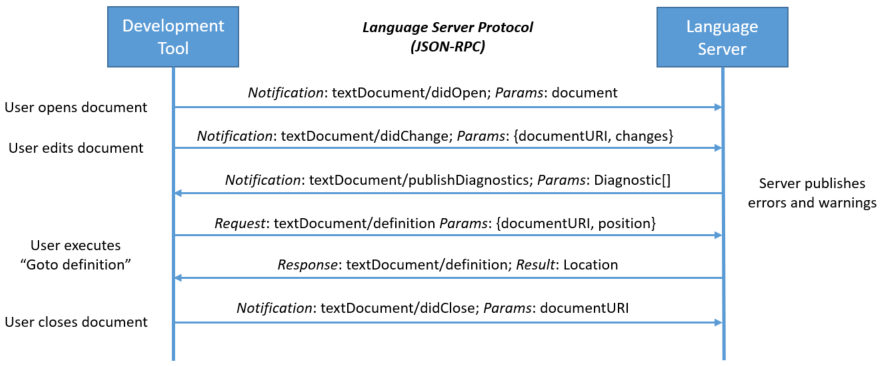
\includegraphics[width=\textwidth]{img/language-server-sequence}
	\caption[LSP session example.]{LSP session example. (source: \url{https://microsoft.github.io/language-server-protocol/overview} )}
	\label{fig04:LSP}
\end{figure}

\begin{figure}
	\centering
	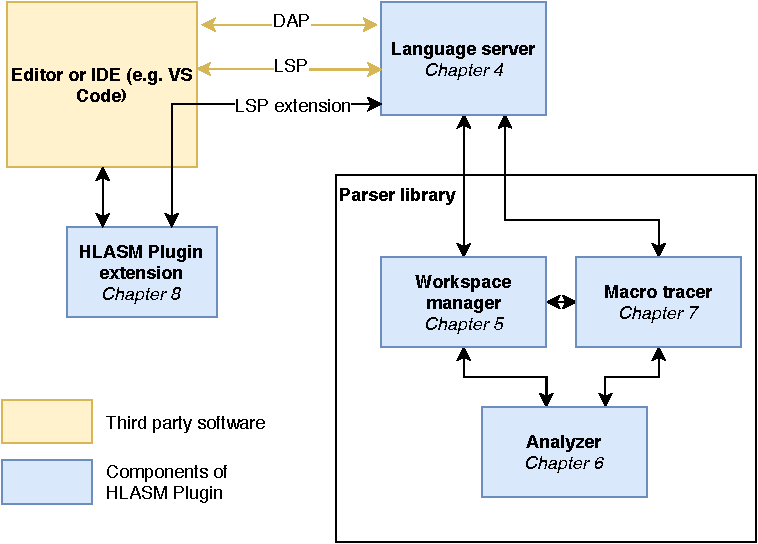
\includegraphics[width=\textwidth]{img/hlasm_architecture}
	\caption{The architecture of HLASM Plugin}
	
	\label{fig04:arch}
\end{figure}

The architecture is based on the way modern code editors and IDEs are extended to support additional languages. We chose to implement Language Server Protocol \footnote{\url{https://microsoft.github.io/language-server-protocol/}} (LSP), which is supported by a majority of contemporary editors.

In LSP, the two parties that communicate are called a \emph{client} and a \emph{language server}. A simple example is displayed in \cref{fig04:LSP} The client runs as a part of an editor. The language server may be a standalone application that is connected to the client by a pipe or TCP. All language-specific user actions (for example the Go to definition command) are transformed into standard LSP messages and are sent to the language server. The language server then analyzes the source code and sends back a response, which is then interpreted and presented to the user in editor-specific way. This architecture makes possible to only have one LSP client implementation for each code editor, which may be reused by all programming languages. And vice versa, every language server may be easily used by any editor that has an implementation of the LSP client.

To add support for HLASM, we have implemented the LSP language server and written a lightweight extension to an editor, which uses an already existing implementation of the LSP client. To implement source code highlighting, we had to extend the protocol with a new notification. This notification is used for transferring information from the language server to the VS Code client, which is extended to highlight code in editor based on the incoming custom notifications.

In this chapter, we further decompose the project into smaller components and describe their relations. The two main components are the parser library and the language server --- an executable application that uses the parser library. An overview of the architecture is pictured in \cref{fig04:arch}. The architecture of whole project is shown in \cref{all_arch}

\section{Language server description}

The responsibility of the language server component is to maintain the LSP session, convert incoming JSON messages and use the parser library to execute them. The functionality includes:
\begin{itemize}
    \item reading LSP messages from either a standard input or TCP and writing responses
    \item parsing JSON RPC to C++ structures, so they can be further used
    \item serializing C++ structures into JSON, so it can be sent back to the client
    \item implementing asynchronous request handling: e.g. when a user makes several consecutive changes to a source code, parsing on every change is not needed
\end{itemize}

\section{Parser library description}

Parser library is the core of the project --- it encapsulates the analyzer, which provides all parsing capabilities, and workspace manager, which keeps track of open files in the editor and manages their dependencies. It has to keep the representation of workspaces and files in the parser library exactly the same as the user sees in the editor. It also starts the analyzer when needed, manages workspace configuration and provides external macro and copy libraries to analyzer.

\subsection{Parser library API}
The parser library API is based on LSP --- every relevant request and notification has a corresponding method in the parsing library.

Firstly, the API implements the LSP notifications that ensure the editor state synchronization. Apart from working with individual files, the LSP also supports workspaces. A workspace is basically just a folder that contains related source codes. The LSP also supports working with multiple workspaces at the same time. We use it when searching for dependencies of HLASM source codes (macros, and copy files).

The parser library needs to have the exact contents of all files in open workspaces. To achieve that, there is a file watcher running in the LSP client that notifies the server when any of the HLASM source files is changed outside of editor. For example, when a user deletes an external macro file, the parser library should react by reporting that it cannot find the macro.

Following is the list of necessary editor state synchronization notifications:
\begin{itemize}
	\item Text synchronization notifications (didOpen, didChange, didClose) that inform the library about files that are currently open in the editor and their exact contents.
	\item DidChangeWorkspaceFolders notification that informs the library when a workspace has been opened or closed.
	\item DidChangeWatchedFiles notification
\end{itemize}

Secondly, the API implements the requests and notifications that provide the parsing results, specifically:
\begin{itemize}
	\item publishDiagnostics notification. A diagnostic is used to indicate a problem with source files, such as a compiler error or a warning. The parser library provides a callback to let the language server know that diagnostics have changed.
	\item Callback for highlighting information provision.
	\item Language feature requests (definition, references, hover, completion), which provide information needed for proper reaction of the editor on user actions.
\end{itemize}

\subsection{Analyzer}

The analyzer is able to process a single HLASM file. The processing includes:
\begin{itemize}
 \item recognition of statements and their parts (lexing and parsing)
 \item interpretation of instructions that should be executed in compile time
 \item a check whether the HLASM source code is well-formed
 \item reporting of problems with the source by producing LSP diagnostics
 \item providing highlighting and LSP information
\end{itemize}

A HLASM file may have dependencies --- other files that define macros or files brought in by the COPY instruction. The dependencies are only discovered during the processing of files, so it is not possible to provide the files beforehand. The analyzer gets a callback that would find a file with specified name, parse its contents and return it as list of parsed statements. 

To sum up, the analyzer has a pretty simple API: it takes the contents of a source file by common string and a callback that can parse external files with specified name. It provides a list of diagnostics linked to the file, highlighting, list of symbol definitions, etc.

\section{Client-side VS Code extension}
\label{arch:client}

The VS Code extension component ensures seamless integration with the editor. Its functions are:

\begin{itemize}
	\item to start the HLASM language server and the LSP client that comes with VS Code, and to create a connection between them.
	\item to implement extension of the LSP protocol for enabling server-side highlighting. The extended client parses the information from the server and uses VS Code API to actually color the text in the editor.
	\item to implement continuation handling --- when the user types something in front of the continuation character, it should stay in place.
\end{itemize}


\section{Macro tracer}
\label{arch:macro}
The macro tracer enables the user to trace the compilation of HLASM source code in a way similar to common debugging. This is the reason why we chose to implement the Debug Adapter Protocol \footnote{\url{https://microsoft.github.io/debug-adapter-protocol/}} (DAP). It is very similar to LSP, so most of the code implementing LSP in the language server component may be reused for both protocols.

The language server component communicates with the macro tracer component in the parser library. Its API mirrors the requests and events of DAP.

Following are the most important DAP features implemented by macro tracer:

\begin{itemize}
	\item launch, continue, next, stepIn and disconnect requests, which allow the user to control the flow of the compilation
	\item SetBreakpoints, which transfers the information about breakpoints that the user has placed in the code
	\item Threads, StackTrace, Scopes and Variables requests to allow the DAP client to retrieve information about the current processing stack (stack of nested macros and copy instructions), available variable symbols and their values
	\item stopped, exited and terminated events to let the DAP client know about state of traced source code
\end{itemize}

The macro tracer communicates with the workspace manager to retrieve the content of the traced files. Afterwards, it starts analyzing the source file in a separate thread and gets callbacks from the analyzer before each statement is processed. In the callback, the tracer puts the thread to sleep and waits for user interaction. During this time, it is possible to retrieve all variable and stack information from the processing to display it to the user.

%probably not needed?
%\include{technologies}
\chapter{Project execution}

\section{Team}
This team consists of five members:

\begin{itemize}
	\item Michal Bali,
	\item Marcel Hruška,
	\item Peter Polák,
	\item Adam Šmelko,
	\item Lucia Tódová.
\end{itemize}

Each team member is responsible for delivering work packages assigned to him or her (see \cref{timeline}). 

\section{Team management} 

For managing the project and team members we use a visual process management system Kanban. Additionally, the project is developed within the environment of Broadcom Inc., which supplies additional project management and supervision. We are attempting to follow the Agile software development guidelines --- our team meets every week with our Broadcom supervisor at stand-ups and discusses the current status of particular tasks with their assignees, reviews progress and plans work for the next week. 

Slack is used for dynamic communication between team members.

\section{Project timeline}
\label{timeline}
The project was split into several milestones and work packages. Presently the milestone \hyperref[milestone_preview]{Preview} has already been reached. Therefore, there is currently a working prototype, and some of the presented work packages are already finished. 

The implementation of the whole project was planned to be accomplished within nine months. The project has been already worked on for four months which has already resulted in completion of milestone M4 Preview. Since most of the architecture, design and planning questions have been answered during the development of the prototype, we do not expect any additional technical or architectural issues at this point. Additionally, the company support from Broadcom Inc. prevents financing and motivation issues. Currently, it seems that it is very probable that the project will be completed as planned. 

The work packages have been assigned to individual team members based on long-term planning. The work packages, their deadlines and assignments are summarized in the \cref{table} and in the overview diagram \ref{fig:gantt-pokus}. 


\newcommand{\WPdef}[3]{\expandafter\def\csname WP#1 \endcsname{\textbf{#2}
		
#3}}
\newcommand{\Mdef}[3]{\expandafter\def\csname M#1 \endcsname{\begin{center} \textbf{#2} \end{center}
		
#3}}
\newcommand{\WPdefe}[2]{\expandafter\def\csname WP#1 \endcsname{\textbf{#2}}}
\newcommand{\Mdefe}[2]{\expandafter\def\csname M#1 \endcsname{\begin{center} \textbf{#2} \end{center}}}


\Mdef{1}{Research and analysis}{}
	\WPdef{1}{HLASM language analysis}
	{analyse and study HLASM specification, available code and discussion with HLASM users}
	\WPdef{2}{Parser libraries research}
	{research and comparison of contemporary lexical and parser libraries (Bison, ANTLR, ...) }
	\WPdef{3}{IDEs research}{research of available IDEs to which would be the HLASM language support integrated }

\Mdef{2}{Hlasm syntax support}{At the second milestone, the plugin is able to parse HLASM syntax, which is shown to the user with server-side highlighting. There is a working implementation of LSP on the server side, which communicates to the VS Code LSP client. The LSP is extended to transfer server-side highlighting information.}

	\WPdefe{4}{Lexer}
	\WPdefe{5}{Parser}
	\WPdefe{6}{LSP implementation}
	\WPdefe{7}{Server-side highlighting}
	
\Mdefe{3}{Detailed specification}{}
	\WPdefe{8}{Detailed specification}{}

\Mdef{4}{Preview}{Output of this milestone is a working demo and its presentation in Broadcom. The parser is able to interpret conditional assembly instructions and expand macros defined within the same source file. It is able to present problems with HLASM source code via LSP diagnostics, and LSP features like Hover or Go to definitions are working with variable symbols.}
	\WPdef{9}{Macro tracer POC}{Proof of concept of the macro tracer by implementation of the Debug Adapter Protocol (see \cref{arch:macro}).}
	\WPdefe{10}{Validation of assembler instructions operands}
	\WPdef{11}{CA instructions}{Interpretation and validation of the conditional assembly instructions.}
	\WPdef{12}{CA expressions}{Evaluation of the conditional assembly expressions. }
	\WPdef{13}{Macro expansion}{Only macros defined within the same file required.}
	\WPdef{14}{Conditional assembly LSP features}{Hover, Go to definition and Find all references for variable symbols}


	
	
\Mdef{5}{Multiple files parsing}{The plugin is able to parse macros from separate files and is able to interpret the COPY instruction. The user experience is improved by continuation handling.}
	\WPdef{15}{Machine expressions}{Evaluation of expressions that are used in assembler and machine instructions.}
	\WPdef{16}{Continuation handling}{VS Code extension functionality to improve working with continuations --- when typing, the continuation at the end of the line should stay in place.}
	\WPdef{17}{External files parsing}{Interpretation of COPY instruction, macro expansion from separate files.}
	\WPdef{18}{File dependencies}{Configuration of processor groups and dependency search (see \cref{LSPFeatures})}
	
\Mdef{6}{Ordinary assembly implementation}{The plugin is able to interpret the EQU and DC instructions and thus evaluate most of ordinary symbols (see \cref{ordinary_resolution}). The acquired values are then used to validate machine instruction operands. Additionally, the user can Go to definition on ordinary symbols and show their values using mouse hover tooltips. }
	\WPdefe{19}{Validation of assembler instructions operands}
	\WPdef{20}{DC instruction}{parsing, validation and length of data definition operand}
	\WPdef{21}{Ordinary symbols}{ordinary assembly implementation}
	\WPdef{22}{Ordinary LSP features}{implementation of support for ordinary symbols}

\Mdef{7}{Finalization}{We reserve some time to polish user experience, finish all components and implement smaller (but important) HLASM features that were not explicitly planned.}
	\WPdefe{23}{Finalization}

\Mdef{8}{Feature testing}{After the M8 milestone, the software should be well tested, stable and able to run seamlessly on any major platform.}
	\WPdefe{24}{Testing}
	\WPdef{25}{Multi-platform deployment}{Deployment on Windows, Linux and Mac OS}
	\WPdefe{26}{Code coverage}
	\WPdef{27}{Benchmark}{Creation of a performance measuring tool that measures how much time the parser needs to analyze a file. It also measures number of processed lines.}
	
\Mdefe{9}{Documentation}
	\WPdefe{28}{Documentation}
	
\Mdefe{10}{Final presentation}
	\WPdefe{29}{Final presentation}

\newcommand{\M}[2]{\multirow{#1}{0.6cm}{\centering M#2}}
\newcommand{\Md}[2]{\multirow{#1}{7cm}{\csname M#2 \endcsname}}
\newcommand{\WP}[2]{\multirow{#1}{1cm}{\centering WP#2}}
\newcommand{\WPd}[2]{\multirow{#1}{7cm}{\csname WP#2 \endcsname}}



\newpage
\begin{landscape}
\begin{longtable}{ccccl}
	\caption{The milestones and work packages organisation}
\label{table}   \\ \toprule
	            \textbf{Ms.}             & \textbf{Milestone description} & \textbf{WP} & \textbf{Work package description} & \textbf{Assignees} \\ \midrule
	             \M{12}{1}               &           \Md{12}{1}           &  \WP{4}{1}  &            \WPd{4}{1}             &                    \\
	                                     &                                &             &                                   & Adam               \\
	                                     &                                &             &                                   & Marcel             \\
	                                     &                                &             &                                   &                    \\
	                                     &                                &             &                                   &                    \\
	                                     &                                &  \WP{4}{2}  &            \WPd{4}{2}             & Peter              \\
	                                     &                                &             &                                   &                    \\
	                                     &                                &             &                                   &                    \\
	                                     &                                &             &                                   &                    \\
	                                     &                                &             &                                   &                    \\
	                                     &                                &  \WP{4}{3}  &            \WPd{4}{3}             &                    \\
	                                     &                                &             &                                   & Lucia              \\
	                                     &                                &             &                                   & Michal             \\
	                                     &       Deadline: month 1        &             &                                   &                    \\ \midrule
	              \M{13}{2}               &           \Md{8}{2}            &  \WP{2}{4}  &            \WPd{2}{4}             & Lucia              \\
	                                     &                                &             &                                   & Peter              \\
	                                     &                                &             &                                   &                    \\
	                                     &                                &  \WP{2}{5}  &            \WPd{2}{5}             & Adam               \\
	                                     &                                &             &                                   & Marcel             \\
	                                     &                                &             &                                   &                    \\
	                                     &                                &  \WP{3}{6}  &            \WPd{3}{6}             &                    \\
	                                     &                                &             &                                   & Michal             \\
	                                     &                                &             &                                   &                    \\
	                                     &                                &  \WP{3}{7}  &            \WPd{3}{7}             &                    \\
	                                     &                                &             &                                   &  Marcel            \\
	                                     &                                &             &                                   &                    \\
	                                     &      Deadline: month 2         &             &                                   &                    \\ \midrule \newpage \midrule
	              \M{4}{3}               &           \Md{4}{3}            & \WP{4}{8}   &            \WPd{4}{8}             &                    \\
	                                     &                                &             &                                   & all                \\
	                                     &                                &             &                                   &                    \\
	                                     &       Deadline: month 3        &             &                                   &                    \\ \midrule
	             \M{24}{4}               &           \Md{24}{4}           &  \WP{4}{9}  &            \WPd{4}{9}             &                    \\
	                                     &                                &             &                                   & Michal             \\
	                                     &                                &             &                                   &                    \\
	                                     &                                &             &                                   &                    \\
	                                     &                                & \WP{4}{10}  &            \WPd{4}{10}            &                    \\
	                                     &                                &             &                                   & Lucia              \\
	                                     &                                &             &                                   &                    \\
	                                     &                                &             &                                   &                    \\
	                                     &                                & \WP{4}{11}  &            \WPd{4}{11}            &                    \\
	                                     &                                &             &                                   & Adam               \\
	                                     &                                &             &                                   &                    \\
	                                     &                                &             &                                   &                    \\
	                                     &                                & \WP{4}{12}  &            \WPd{4}{12}            &                    \\
	                                     &                                &             &                                   & Peter              \\
	                                     &                                &             &                                   &                    \\
	                                     &                                &             &                                   &                    \\
	                                     &                                & \WP{4}{13}  &            \WPd{4}{13}            &                    \\
	                                     &                                &             &                                   & Adam               \\
	                                     &                                &             &                                   &                    \\
	                                     &                                &             &                                   &                    \\
	                                     &                                & \WP{4}{14}  &            \WPd{4}{14}            &                    \\
	                                     &                                &             &                                   & Marcel             \\
	                                     &                                &             &                                   &                    \\
	                                     &                                &             &                                   &                    \\
	                                     &       Deadline: month 4        &             &                                   &                    \\ \midrule \newpage \midrule
	             \M{18}{5}               &           \Md{16}{5}           & \WP{4}{15}  &            \WPd{4}{15}            &                    \\
	                                     &                                &             &                                   & Michal             \\
	                                     &                                &             &                                   &                    \\
	                                     &                                &             &                                   &                    \\
	                                     &                                & \WP{6}{16}  &            \WPd{6}{16}            &                    \\
	                                     &                                &             &                                   & Marcel             \\
	                                     &                                &             &                                   &                    \\
	                                     &                                &             &                                   &                    \\
	                                     &                                &             &                                   &                    \\
	                                     &                                &             &                                   &                    \\
	                                     &                                & \WP{4}{17}  &            \WPd{4}{17}            &                    \\
	                                     &                                &             &                                   & Adam               \\
	                                     &                                &             &                                   &                    \\
	                                     &                                &             &                                   &                    \\
	                                     &                                & \WP{3}{18}  &            \WPd{3}{18}            &                    \\
	                                     &                                &             &                                   & Michal             \\
	                                     &        Deadline: month 5       &             &                                   &                    \\ \midrule
	           \M{14}{6}                 &        \Md{12}{6}              & \WP{3}{19}  &            \WPd{3}{19}            &                    \\
	                                     &                                &             &                                   & Lucia              \\
	                                     &                                &             &                                   &                    \\
	                                     &                                & \WP{4}{20}  &            \WPd{4}{20}            &                    \\
	                                     &                                &             &                                   & Michal             \\
	                                     &                                &             &                                   & Peter              \\
	                                     &                                &             &                                   &                    \\
	                                     &                                & \WP{4}{21}  &            \WPd{4}{21}            &                    \\
	                                     &                                &             &                                   &  Peter             \\
	                                     &                                &             &                                   &  Adam              \\
	                                     &                                &             &                                   &                    \\
	                                     &                                & \WP{3}{22}  &            \WPd{3}{22}            &                    \\
	                                     &                                &             &                                   &  Marcel            \\
	                                     &       Deadline: month 7        &             &                                   &                    \\ \midrule \newpage \midrule
	              \M{9}{7}               &           \Md{6}{7}            & \WP{10}{23} &            \WPd{10}{23}           &                    \\
	                                     &                                &             &                                   &                    \\
	                                     &                                &             &                                   &                    \\
	                                     &                                &             &                                   &                    \\
	                                     &                                &             &                                   &  all               \\
	                                     &                                &             &                                   &                    \\
	                                     &                                &             &                                   &                    \\
	                                     &                                &             &                                   &                    \\
	                                     &         Deadline: month 8      &             &                                   &                    \\ \midrule
	             \M{16}{8}               &           \Md{12}{8}           & \WP{3}{24}  &            \WPd{3}{24}            &                    \\
	                                     &                                &             &                                   & all                \\
	                                     &                                &             &                                   &                    \\
	                                     &                                & \WP{4}{25}  &            \WPd{4}{25}            &                    \\
	                                     &                                &             &                                   & Michal             \\
	                                     &                                &             &                                   &                    \\
	                                     &                                &             &                                   &                    \\
	                                     &                                & \WP{3}{26}  &            \WPd{3}{26}            &                    \\
	                                     &                                &             &                                   & Lucia              \\
	                                     &                                &             &                                   &                    \\
	                                     &                                & \WP{6}{27}  &            \WPd{6}{27}            &                    \\
	                                     &                                &             &                                   & Marcel             \\
	                                     &                                &             &                                   &                    \\
	                                     &                                &             &                                   &                    \\
	                                     &                                &             &                                   &                    \\
	                                     &          Deadline: month 9     &             &                                   &                    \\ \midrule
	              \M{3}{9}               &         \textbf{Documentation} & \WP{3}{28}  &            \WPd{3}{28}            &                    \\
	                                     &                                &             &                                   & all                \\
	                                     &          Deadline: month 9     &             &                                   &                    \\ \midrule
	              \M{3}{10}              &  \textbf{Final Presentation}   & \WP{3}{29}  &            \WPd{3}{29}            &                    \\
	                                     &                                &             &                                   & all                \\
	                                     &          Deadline: month 9     &             &                                   &                    \\ \bottomrule
\end{longtable}
\end{landscape}


\begin{landscape}
	\begin{figure}
		\centering
		\tikzstyle{wp}=[anchor=east, font={\small\bf\cool}, inner sep=1mm]
		\tikzstyle{swp}=[anchor=base west, font={\tiny\it}, inner sep=0mm]
		\tikzstyle{month}=[anchor=west, rotate=90]
		\newcommand{\ganttitem}[4]{\node[wp] (#1) at(#2) {#3}; \node[swp] at (#1.east|-#1.base) {#4};}
		\begin{tikzpicture}
		\foreach \wp in {1,...,30} {
			\coordinate (wp\wp) at (0,\wp * -1.2em);
		};
		\foreach \tim in {1,...,9} {
			\coordinate (t\tim) at (\tim * 2cm,0);
			\node[month] at (t\tim) {Month \tim};
			\draw[dotted, thin, draw=black!25] (t\tim) to (t\tim |- wp30); %sync with previous
		};
		
		
		\draw[draw=black!25] (t3) to (t3 |- wp27); %sync with previous
		\node[month] at (t3|-wp30) {today};
		
		\ganttitem{ider}{t1|-wp3}{IDEs research}{Lucia, Michal};
		\ganttitem{pare}{t1|-wp2}{Parser libraries research}{Peter};
		\ganttitem{hlas}{t1|-wp1}{HLASM analysis}{Adam, Marcel};
		
		\ganttitem{lex}{t2|-wp4}{Lexer}{Lucia, Peter};
		\ganttitem{lex}{t2|-wp5}{Parser}{Adam, Marcel};
		\ganttitem{lsppoc}{t2|-wp6}{LSP implementation}{Michal}
		\ganttitem{vspoc}{t2|-wp7}{Server-side highlighting}{Marcel}

		
		\ganttitem{lex}{t3|-wp8}{Detailed specification}{all};
		
		
		\ganttitem{vspoc}{t4|-wp9}{Macro tracer POC}{Michal}
		\ganttitem{lex}{t4|-wp10}{Validation of assembler instructions operands}{Lucia};
		\ganttitem{lex}{t4|-wp11}{CA instructions}{Adam};
		\ganttitem{lex}{t4|-wp12}{CA expressions}{Peter};
		\ganttitem{lex}{t4|-wp13}{Macro expansion}{Adam};
		\ganttitem{lex}{t4|-wp14}{Conditional assembly LSP features}{Marcel};
		
		
		\ganttitem{lex}{t5|-wp15}{Machine expressions}{Michal};
		\ganttitem{lex}{t5|-wp16}{Continuation handling}{Marcel};
		\ganttitem{lex}{t5|-wp17}{External files parsing}{Adam};
		\ganttitem{lex}{t5|-wp18}{File dependencies}{Michal};
		
		
		\ganttitem{lex}{t7|-wp19}{Validation of assembler instructions operands}{Lucia};
		\ganttitem{lex}{t7|-wp20}{DC instruction}{Michal, Peter};
		\ganttitem{lex}{t7|-wp21}{Ordinary symbols}{Peter, Adam};
		\ganttitem{lex}{t7|-wp22}{Ordinary LSP features}{Marcel};
		
		
		\ganttitem{lex}{t8|-wp23}{Finalization}{all};
		
		\ganttitem{lex}{t9|-wp24}{Testing}{all};
		\ganttitem{lex}{t9|-wp25}{Multi-platform deployment}{Michal};
		\ganttitem{lex}{t9|-wp26}{Code coverage}{Lucia};
		\ganttitem{lex}{t9|-wp27}{Benchmark}{Marcel};
		
		\ganttitem{lex}{t9|-wp28}{Documentation}{all};
		\ganttitem{lex}{t9|-wp29}{Final presentation}{all};
		
		
		\end{tikzpicture}
		\caption{Work packages overview}
		\label{fig:gantt-pokus}
	\end{figure}
\end{landscape}











\iffalse

\bms
\itemm Research and analysis \deadline{2}{2}

\small The output of this milestone should be deeper knowledge and understanding of HLASM language, selection of parser library and target IDE.
HLASM is complicated language, hence the choice of right parser library is vital for further development. Also important is to choose IDE in witch would be the language support integrated.

\bwp
\itemwp HLASM language analysis \people{Adam, Marcel}
\tiny study and analysis of HLASM documentation, available code and discussion with HLASM users

\itemwp Parser libraries research \people{Peter}
\tiny research and comparison of contemporary lexical and parser libraries (Bison, ANTLR, ...) 

\itemwp IDEs research \people{Michal, Lucia}
\tiny research of available IDEs to which would be the HLASM language support integrated
\eenum


\itemm Parser prototype \deadline{3}{2}

\small With knowledge and selected tools from previous milestone, this milestone should output first prototype of parser.

\bwp
\itemwp Lexer \people{Lucia, Peter}
\itemwp Parser \people{Adam, Marcel}
\eenum


\itemm IDE integration prototype \deadline{3}{1}

\small In this milestone should be accomplished integration of the parser to the selected IDE.

\bwp
\itemwp LSP POC \people{Michal}
\tiny proof of concept of the Language Server Protocol (LSP) implementation (see chapter \hyperref[arch]{Architecture})

\itemwp VS Code client POC \people{Michal}
\tiny proof of concept of the \hyperref[arch:client]{VS Code client}

\itemwp Debugger POC \people{Michal}
\tiny proof of concept of the Debug Adapter Protocol (see \ref{arch:macro})
\eenum





\itemm \label{milestone_preview} Preview \deadline{4}{2}

\small Output of this milestone is working demo and its presentation in Broadcom. To accomplish this, several essential WPs must be done.

\bwp
\itemwp Client semantic highlighting \people{Marcel}
\tiny implementation of semantic highlighting in the IDE

\itemwp Assembler checker \people{Lucia}
\tiny validation of assembler instruction operands

\itemwp Conditional assembly instructions \people{Adam}
\tiny processing of conditional assembly instructions inside the Analyzer

\itemwp Conditional assembly expressions \people{Peter}
\tiny evaluation of conditional assembly expression 

\itemwp Macro expansion \people{Adam}
\tiny processing of macros (expansion)

\itemwp Conditional assembly LSP features \people{Marcel}
\tiny Hover, Go to definition and Find all references for variable symbols


\eenum




\itemm Detailed specification \deadline{6}{1}
\bwp
\itemwp Detailed specification \people{all}
\eenum


\itemm Features \deadline{7}{4}

\small Addition of other important features.

\bwp

\itemwp Machine expressions \people{Michal}
\tiny expressions that are used in assembler and machine instructions

\itemwp Machine instruction checker \people{Lucia}
\tiny validation of machine instruction operands

\itemwp DC instruction \people{Michal, Peter}
\tiny parsing, validation and length of data definition operand

\itemwp Copy instruction \people{Adam}
\tiny external files include

\itemwp Client-server continuation handling \people{Marcel}
\tiny implementation of support for continuation (see \cref{Continuation})

\itemwp Diagnostics \people{Lucia}
\tiny errors and warnings reporting polishing

\itemwp Ordinary LSP features \people{Marcel}
\tiny implementation of support for ordinary symbols

\itemwp Ordinary symbols \people{Adam, Peter}
\tiny ordinary assembly implementation
\eenum

\itemm Finalization \deadline{8}{1}

\small After this milestone should be all components finalized. 

\bwp
\itemwp Finalization \people{all}
\eenum

\itemm Feature testing \deadline{9}{2}

\small Goal of this milestone is to test, polish and benchmark all code from previous milestones.

\bwp
\itemwp Testing \people{all}

\itemwp Multiplatform deployment \people{Michal}
\tiny deployment on platforms Windows, Linux and Mac OS

\itemwp Code coverage \people{Lucia}

\itemwp Benchmarking \people{Marcel}
\eenum

\itemm Documentation \deadline{9}{1}

\small Goal is to assembly a complete documentation for whole work.

\bwp
\itemwp Documentation \people{all}
\eenum

\itemm Final presentation \deadline{9}{0}
\bwp
\itemwp Final presentation \people{all}
\eenum
\eenum



\newgeometry{a4paper,left=1in,right=1in,top=1in,bottom=1in,nohead}

\begin{landscape}
	\begin{figure}
		\centering
		\begin{ganttchart}[vgrid={draw=none, dotted}, x unit = 1.2cm]{1}{12}
		
		\gantttitlelist{"1. month", "2. month", "3. month"}{4} \\
		\gantttitlelist{1,...,12}{1} \\
		
		\ganttbar{HLASM language analysis (A \& Ma)}{1}{8} \\
		\ganttbar{Parser libraries research (P)}{1}{4}\\
		\ganttbar{IDEs research (L \& Mi)}{1}{4}\\
		
		\ganttbar{LSP POC (Mi)}{5}{8} \\
		\ganttbar{VSCode client POC(Mi)}{5}{8}\\
		\ganttbar{Lexer (L \& P)}{5}{10}\\
		\ganttbar{Parser (A \& Ma)}{5}{12}\\
		
		\ganttbar{Client semantic highlighting (Ma)}{9}{12}\\
		\ganttbar{Assembler checker (L)}{9}{12}\\
		\ganttbar{Debugger POC (Mi)}{9}{12}\\
		\ganttbar{Conditional assembly instructions (A)}{9}{12}\\
		\ganttbar{Conditional assembly expressions (P) $\rightarrow$}{11}{12}\\
		
		\ganttvrule[vrule offset=0.8]{today}{12}
		
		\end{ganttchart}
    \caption{Tasks for months 1 -- 3}
	\label{fig:gantt1}
	\end{figure}
\end{landscape}


\begin{landscape}
	\begin{figure}
		\centering
		\begin{ganttchart}[vgrid={draw=none, dotted}, x unit = 1.2cm]{1}{12}
			
			\gantttitlelist{"4. month", "5. month", "6. month"}{4} \\
			\gantttitlelist{13,...,24}{1} \\
			\ganttbar{$\rightarrow$ Conditional assembly expressions (P)}{1}{2}\\
			\ganttbar{Macro expansion (A)}{1}{4}\\
			\ganttbar{Conditional assembly LSP features (Ma)}{1}{4}\\
			\ganttbar{Machine expressions (Mi)}{1}{4}\\
			
			\ganttmilestone{Demo presentation}{4}\\
			
			\ganttbar{Machine instruction checker (L)}{1}{12}\\
			\ganttbar{DC instruction (Mi \& P)}{3}{12}\\
			
			\ganttbar{Copy instruction (A)}{5}{8}\\
			\ganttbar{Client-server continuation handling (Ma)}{5}{8}\\
			
			\ganttbar{Diagnostics (L)}{9}{12} \\
			\ganttbar{Ordinary LSP features (Ma)}{9}{12}\\
			\ganttbar{Ordinary symbols (A \& P) $\rightarrow$}{9}{12}
			
			
			
		\end{ganttchart}
		\caption{Tasks for months 4 -- 6}
		\label{fig:gantt2}
	\end{figure}
\end{landscape}

\begin{landscape}
	\begin{figure}
		\centering
		\begin{ganttchart}[vgrid={draw=none, dotted}, x unit = 1.2cm]{1}{12}
			
			\gantttitlelist{"7. month", "8. month", "9. month"}{4} \\
			\gantttitlelist{25,...,36}{1} \\
			
			
			\ganttbar{$\rightarrow$ Ordinary symbols (A \& P)}{1}{4}\\
			\ganttbar{Multiplatform deployment (Mi)}{1}{4}\\
			\ganttbar{Benchmarking (Ma)}{1}{4}\\
			\ganttbar{Code coverage (L)}{1}{8}\\
			
			\ganttbar{Testing (all)}{5}{12}\\
			
			\ganttbar{Documentation (all)}{9}{12}\\
		
			
			\ganttvrule[vrule offset=0.2]{today}{1}
			
		\end{ganttchart}
		\caption{Tasks for months 7 -- 9}
		\label{fig:gantt3}
	\end{figure}
\end{landscape}

\restoregeometry
\fi





\end{document}
